\documentclass[conference]{IEEEtran}
\usepackage{times}

% numbers option provides compact numerical references in the text. 
\usepackage[numbers]{natbib}
\usepackage{multicol}
\usepackage[bookmarks=true]{hyperref}
\usepackage{pgfplots}
\usepackage{fontspec}
\pgfplotsset{compat=1.18}

\begin{document}

% paper title
\title{Language, Decoded: Exploring the Impact of Native-Language Code on Multilingual Models}

\author{
\authorblockN{Tom Sherborne}
\authorblockA{Cohere\\
Edinburgh, Scotland, UK\\
tomsherborne@cohere.com}
\and
\authorblockN{Madi Edgar}
\authorblockA{Legesher\\
Dubai, UAE\\
madi@legesher.com}
\and
\authorblockN{Saad Ahmed Bazaz}
\authorblockA{Grayhat\\
Islamabad, PK\\
bazaz@grayhat.studio}
\and
\authorblockN{Rashik Shahjahan}
\authorblockA{Independent\\
Toronto, CA\\
rashikshahjahan@protonmail.com}
\and
\authorblockN{Khojasteh Z. Mirza}
\authorblockA{The Friedman Brain Institute\\
New York, USA\\
khojasteh.mirza@mssm.edu}
\and
\authorblockN{Sarah Jawaid}
\authorblockA{Grayhat\\
Karachi, PK\\
sarah.jawaid@grayhat.studio}
\and
\authorblockN{Rafay Mustafa}
\authorblockA{Tkxel\\
Lahore, PK\\
rafaym30@gmail.com}
\and
\authorblockN{Sohaib Ahmed Bazaz}
\authorblockA{Grayhat\\
Islamabad, PK\\
sohaib.bazaz@grayhat.studio}
}

\maketitle

\begin{abstract}
Large language models (LLMs) have shown remarkable capabilities in multilingual tasks, but the impact of training on code written in native languages remains underexplored. This paper investigates whether continued pre-training of multilingual models on native-language code improves their reasoning, world knowledge, and instruction following compared to English code or no code training. We conduct a systematic experiment using Tiny Aya, training it on various conditions of code data in Chinese, Spanish, and Urdu. Evaluations on MGSM, X-CSQA, and XNLI benchmarks reveal that native-language code provides language-specific benefits, with keyword-swapped code showing initial gains for Chinese XNLI. However, deeper analysis reveals that XNLI accuracy at this model scale primarily reflects label bias shifts rather than improved natural language inference capability. Urdu keyword training causes code leakage into evaluation outputs, while mathematical reasoning shows no improvement across any condition. Our findings highlight both the potential and limitations of multilingual code fine-tuning for small-scale models.
\end{abstract}

\IEEEpeerreviewmaketitle

\section{Introduction}

Multilingual large language models (LLMs) are increasingly vital for global applications, yet their performance often lags in non-English languages due to imbalanced training data. Recent research has demonstrated that training on code can enhance reasoning and instruction-following abilities in LLMs \cite{code_or_not}. However, the extent to which this phenomenon generalizes to other languages remains underexplored.

This paper explores the hypothesis that code composed in native languages carries unique cultural and linguistic signals that improves native language performance beyond what is achievable using English code. We investigate this through controlled experiments on TinyAya, a multilingual LLM, using an ``experimental ladder'' of conditions that progressively introduce native-language elements.

Our core research question is: \textit{Does multilingual code improve Tiny Aya's reasoning, world knowledge, and instruction following?} We target Chinese (zh), Spanish (es), and Urdu (ur), evaluating on MGSM for math reasoning, X-CSQA for commonsense reasoning, and XNLI for natural language inference.

The experiment isolates variables: from no training (baseline) to English code, keyword-swapped code, mixed native sources, and strictly native code. This ladder design allows us to measure incremental benefits of native-language exposure.

Our results show that Chinese keyword-swapped code yields a +6.2 percentage point improvement on Chinese XNLI, representing a significant shift in label bias. However, this improvement does not generalize to Spanish or Urdu, and deeper output analysis reveals the model collapses XNLI to binary classification, never predicting the ``neutral'' category. Mathematical reasoning shows no improvement across any condition, and Urdu keyword training causes code leakage into evaluation outputs. These findings suggest that while native-language code can influence model behavior, the effects are language-specific and should be interpreted with attention to benchmark limitations at small model scales.

\section{Literature Review}


\subsection{Multilingual LLMs and Evaluation Benchmarks}
Large multilingual Transformer models have seen rapid development. For example, mT5 \cite{xue-etal-2021-mt5} was trained on a Common Crawl corpus covering 101 languages, achieving state-of-the-art results on many multilingual tasks. More recently, Tiny Aya \cite{salamanca2026tinyayabridgingscale} showed that even a compact 3.35B-parameter model can match larger models by training on 70 languages, yielding state-of-the-art translation and understanding performance across diverse languages. Standard benchmarks reveal persistent gaps in non-English performance. XNLI \cite{conneau-etal-2018-xnli} extended the MultiNLI corpus to 15 languages (including low-resource ones like Urdu) and demonstrated that direct multilingual models lag behind translation-based approaches.  

Researchers have also created multilingual reasoning benchmarks to stress-test models. Key examples include: 

\subsubsection{MGSM \cite{msgm}}
A multilingual grade-school math benchmark with 250 word problems translated into 10 typologically diverse languages. Chain-of-thought prompting enabled high accuracy, and even underrepresented languages showed surprisingly strong reasoning abilities.

\subsubsection{X-CSQA \cite{lin-etal-2021-common}}
The CommonsenseQA dataset translated into 14 languages (along with X-CODAH). This enables cross-lingual commonsense QA evaluation and underlines the need for better multilingual commonsense reasoning.

\subsubsection{XNLI \cite{conneau-etal-2018-xnli}}
A natural language inference benchmark in 15 languages, showing that models trained on one language (English) cannot simply transfer to others without substantial performance loss.

These datasets highlight that models frequently struggle on non-English inputs. For example, multilingual LLMs typically score lower on MGSM and X-CSQA in underrepresented languages than in English. \citeauthor{lin-etal-2021-common} improved multilingual commonsense reasoning with techniques like contrastive pretraining, but this work – like others – did not incorporate code-based training. 
\subsection{Code as a Training Signal in LLMs}
The idea of using code to improve LLM capabilities has gained traction. \citeauthor{code_or_not} performed controlled experiments comparing models pretrained with and without English code. They found that adding code strongly benefits natural language tasks: models pretrained with code showed up to +8.2\% relative gains on language reasoning tasks, +4.2\% on world knowledge, and a +6.6\% win-rate improvement, while code performance itself jumped 12×. These gains held across model scales (470M to 2.8B parameters) and architectures, indicating code data is a “critical building block for generalization” beyond coding tasks. However, the implementation only used English (mostly Python) code in their pretraining.  

Recent work has identified stark weaknesses when code models see non-English inputs. \citeauthor{li2025bridginglanguagegapenhancing} evaluated code-generation LLMs on the MBPP benchmark translated into several languages. They observed significant disparities in code quality for non-English prompts (even though the problem statements were semantically identical). To bridge this gap, \citeauthor{li2025bridginglanguagegapenhancing} proposed a novel zero-shot cross-lingual projection method: a multilingual encoder (LASER) maps any input language into a joint embedding space, which is then projected into the LLM's input space. By training this projection only on English data, they achieved substantial improvements on the translated MBPP benchmark, effectively empowering an English-trained LLM to generate correct code from non-English prompts.  

\citeauthor{kocetkov2022stack3tbpermissively} further document the English dominance in code corpora. They note that in The Stack (a 3TB permissive code dataset), 94\% of code comments are English. This imbalance correlates with performance drops: one study found that using Chinese instructions (instead of English) led to >13\% lower code-generation accuracy. \cite{nishigata-etal-2025-non} These findings underscore that code-focused LLMs inherit the same cross-lingual biases seen in text-only models. \citeauthor{monteiro2024multilingual} took a step toward evaluation by building M²CRB, a multilingual code-search benchmark with text-code pairs in Spanish, Portuguese, German, and French (paired with Python/Java/JS snippets). They show that by combining English–code data with translation corpora, models can surprisingly generalize to “unseen” language–code pairs.

Training data imbalance is the primary reason LLMs show weaker reasoning in non-English languages \cite{huang2024mindmerger}. English dominates pretraining corpora (50-90\% of tokens), so models internalize reasoning patterns like chain-of-thought or multi-step logic far better in English than in low-resource languages \cite{rohera2025better}. Given that prior work \cite{code_or_not} demonstrated English code training improves reasoning capabilities, this study examines whether the same principle extends to resource-constrained languages—specifically, whether training on code written in Chinese, Spanish, or Urdu can enhance native-language reasoning and instruction following.

\subsection{Programming-Language Localization and Native-Code Initiatives}
Beyond LLMs, there is growing interest in localizing programming languages themselves. \citeauthor{localization_framework} outline a 12-aspect framework for fully localizing a language – covering keywords, numerals, word order, etc. – to reduce entry barriers for non-English speakers. Building on this idea, \citeauthor{multilingual_pl} developed UniversalPython, a Python transpiler that lets users write Python with keywords in their own language. They demonstrated an “Urdu Python” variant, showing how programming can be made accessible to Urdu speakers. Similarly, the Legesher project \cite{Edgar_Legesher_Because_language_2026} provides tools and language packs to write Python code using native-language keywords and docs. According to Legesher documentation, its language-localized environment “lets developers write code using keywords, syntax, and documentation in their own language—without changing how the program runs”. These efforts suggest native-language code carries cultural and linguistic context that may be beneficial if absorbed by models.  

\subsection{Gaps and Our Focus}
Prior work has shown that code is a powerful training signal for LLMs and that multilingual benchmarks expose weaknesses in non-English contexts. Localization research indicates rich opportunities in coding with native languages. However, no study has systematically compared the impact of training on native-language code versus English code. In particular, it is unknown whether fine-tuning a multilingual LLM on code written in Chinese, Spanish, Urdu, etc., confers advantages beyond simple language exposure. Our work fills this gap by evaluating how native-language programming data affects multilingual reasoning and instruction following compared to English-only code training.  

In short, while prior work has explored whether code helps LLMs, we investigate how the language of the code matters. By comparing fine-tuning on English code versus native-language code, our study addresses a novel question at the intersection of code and cross-lingual learning. 

\begin{table*}[h]
  \centering
  \caption{Data Sources and Quality Levels}
  \begin{tabular}{|p{5cm}|p{5cm}|p{2.5cm}|}
    \hline
    \textbf{Source} & \textbf{Description} & \textbf{Quality} \\
    \hline
    The Stack (target language subset) & Real-world multilingual code & High \\
    \hline
    Native programming languages & Wenyan, Qi, Latino, etc. & High \\
    \hline
    Legesher-transpiled code & Python converted to target language syntax & Medium \\
    \hline
    Localized comments only & English code with translated comments & Low \\
    \hline
\end{tabular}
\end{table*}

\section{Methodology}
We employ an experimental ladder design to isolate the impact of native-language code on multilingual LLM performance. Our base model is \texttt{CohereLabs/tiny-aya-base}, a 3.35B-parameter causal language model. Rather than full continued pretraining, we adapt the model with parameter-efficient QLoRA so that all conditions can be trained under the same constrained compute budget on Kaggle T4 GPUs.

\subsection{Data Curation}
Data was curated according to a quality hierarchy designed to capture progressively richer linguistic signals in code:

\begin{itemize} 
\item \textbf{Fully native code} (best): Code written entirely in the target language, including identifiers, syntax adaptations, and comments. 
\item \textbf{Function names, variable names, and comments in target language} (medium): Code retains English syntax but incorporates localized naming and documentation. 
\item \textbf{Comments only in target language} (acceptable): Code remains structurally in English, but includes localized explanations. 
\end{itemize}

Datasets for each language were constructed from multiple sources:

\begin{itemize} \item Code extracted from \textbf{The Stack} dataset \cite{kocetkov2022stack3tbpermissively} for the target language. \item Native programming languages in the target languages (e.g., Wenyan \cite{Huang_wenyan_A_Programming_2019} and Qi \cite{Yang_Qi_A_Lightweight_2021} for Chinese via GitHub and Gitee; Latino \cite{Lenguaje_Latino_Contributors_Latino_Lenguaje_de_2024} programming language for Spanish via GitHub). \item Transpiled Python programs into the target language using Legesher \cite{Edgar_Legesher_Because_language_2026}. \end{itemize}

Each language dataset consisted of a mixture of these sources, ensuring diversity in linguistic and structural representation. We filtered code for basic validity, removed obvious duplicates, and used static code analysis to verify quality and correctness where possible, particularly for the fully native and transpiled code conditions. For training, each sample is treated as a plain code document and serialized through the model tokenizer without adding task-specific supervision.

The resulting datasets were uploaded to Hugging Face \cite{legesher_language_decoded} for accessibility during training and evaluation.

\subsection{Experimental Conditions}
The conditions form a progressive ladder, each building on the previous to test incremental hypotheses:

\begin{enumerate}
\item \textbf{Baseline}: No training, evaluating base model performance.
\item \textbf{Condition 1 - English Code}: Trained on English Python from The Stack Dedup.
\item \textbf{Condition 2 - Keyword-Swapped}: Per-language training on Legesher-transpiled Python with native keywords (e.g., \texttt{if} $\rightarrow$ \texttt{如果} in Chinese).
\item \textbf{Condition 3 - Mixed Native Sources}: Per-language blend of transpiled Python, native programming languages (e.g., Wenyan for Chinese), and community code.
\end{enumerate}

\subsection{Training Procedure}
All trainable variants were produced with the same QLoRA recipe to keep the comparison focused on data differences rather than optimizer changes. We load Tiny Aya in 4-bit mode and attach LoRA adapters to the attention and MLP projection layers (\texttt{q\_proj}, \texttt{k\_proj}, \texttt{v\_proj}, \texttt{o\_proj}, \texttt{gate\_proj}, \texttt{up\_proj}, \texttt{down\_proj}) with rank $r=16$, $\alpha=32$, and zero dropout.

Training was implemented with Unsloth and TRL on Kaggle T4 GPUs. The training script sets maximum sequence length to 1024, uses per-device batch size 8 with gradient accumulation 1, and optimizes with paged AdamW 8-bit. We use a cosine learning-rate schedule with 5\% warmup, learning rate $2\times10^{-4}$, weight decay 0.01, max gradient norm 1.0, and gradient checkpointing to stay within the memory limits of 4-bit fine-tuning.

Before optimization, each dataset is pretokenized by applying the Tiny Aya tokenizer to the \texttt{code} field with truncation to 1024 tokens. Training then optimizes the standard causal language modeling objective for one epoch per condition. The training configuration is otherwise held fixed across English-code, keyword-swapped, and mixed-native runs so that any downstream differences can be attributed to the training data rather than to changes in optimization.

To test whether large curated corpora were necessary at this model scale, we trained English-code baselines using both the full English dataset and a 5K-file subset. The small gap between these runs (reported in Section~IV) indicates that the observed downstream effects are not driven solely by corpus size.

\subsection{Evaluation}
We evaluate on MGSM (250 examples), X-CSQA ($\sim$1K examples), and XNLI ($\sim$5K examples) in English, Chinese, Spanish, and Urdu. Each evaluation uses dual prompts: English and language-specific. Benchmarks measure math reasoning, commonsense reasoning, and natural language inference, respectively.

\section{Results}
We present results from controlled experiments comparing baseline performance against code fine-tuned models. Table~\ref{tab:native_results} shows native prompt results, while Table~\ref{tab:english_results} shows English prompt results across all conditions.

\begin{table*}[t]
\centering
\caption{Native Prompt Results (language-specific prompt + target-language data)}
\label{tab:native_results}
\begin{tabular}{|l|c|c|c|c|c|c|c|c|c|}
\hline
\textbf{Condition} & \textbf{MGSM zh} & \textbf{MGSM es} & \textbf{MGSM ur} & \textbf{XNLI zh} & \textbf{XNLI es} & \textbf{XNLI ur} & \textbf{CSQA zh} & \textbf{CSQA es} & \textbf{CSQA ur} \\
\hline
Baseline & 6.0\% & 5.6\% & 3.2\% & 35.8\% & 49.1\% & 38.1\% & 52.1\% & 52.4\% & 40.0\% \\
Cond 1 (en full) & 4.4\% & 6.4\% & 2.8\% & 36.5\% & 48.0\% & 36.9\% & 52.4\% & 53.3\% & 40.6\% \\
Cond 1 (en 5K) & 3.6\% & 5.6\% & 2.8\% & 36.1\% & 47.3\% & 36.8\% & 52.3\% & 53.3\% & 40.7\% \\
Cond 2-zh & 6.0\% & 6.8\% & 4.4\% & 42.3\% & 43.1\% & 36.2\% & 52.9\% & 53.4\% & 41.0\% \\
Cond 2-es & 3.2\% & 5.6\% & 4.4\% & 34.2\% & 44.5\% & 33.3\% & 52.2\% & 53.4\% & 39.8\% \\
Cond 2-ur & 3.2\% & 6.8\% & 3.2\% & 34.6\% & 48.8\% & 37.7\% & 52.4\% & 53.6\% & 38.2\% \\
Cond 3-zh & 7.2\% & 4.0\% & 3.2\% & 35.8\% & 41.6\% & 34.0\% & 54.5\% & 52.8\% & 42.2\% \\
\hline
\end{tabular}
\end{table*}

\begin{table*}[t]
\centering
\caption{English Prompt Results (English prompt + target-language data)}
\label{tab:english_results}
\begin{tabular}{|l|c|c|c|c|c|c|c|c|c|}
\hline
\textbf{Condition} & \textbf{MGSM zh} & \textbf{MGSM es} & \textbf{MGSM ur} & \textbf{XNLI zh} & \textbf{XNLI es} & \textbf{XNLI ur} & \textbf{CSQA zh} & \textbf{CSQA es} & \textbf{CSQA ur} \\
\hline
Baseline & 6.8\% & 7.2\% & 6.0\% & 46.4\% & 51.2\% & 40.9\% & 52.3\% & 53.8\% & 41.2\% \\
Cond 1 (en full) & 8.0\% & 9.2\% & 6.0\% & 47.1\% & 52.2\% & 41.2\% & 51.2\% & 53.4\% & 42.1\% \\
Cond 1 (en 5K) & 8.4\% & 9.6\% & 6.4\% & 47.0\% & 52.2\% & 41.8\% & 51.7\% & 53.5\% & 42.2\% \\
Cond 2-zh & 7.2\% & 10.0\% & 6.8\% & 46.9\% & 52.7\% & 40.2\% & 51.3\% & 53.1\% & 42.2\% \\
Cond 2-es & 7.2\% & 10.8\% & 6.8\% & 51.4\% & 48.0\% & 36.3\% & 51.5\% & 52.2\% & 40.8\% \\
Cond 2-ur & 6.0\% & 10.8\% & 7.2\% & 52.0\% & 52.1\% & 40.0\% & 51.4\% & 54.3\% & 39.8\% \\
Cond 3-zh & 8.4\% & 10.0\% & 8.8\% & 51.1\% & 51.4\% & 36.9\% & 53.8\% & 55.6\% & 43.3\% \\
\hline
\end{tabular}
\end{table*}

\subsection{Key Findings}

\subsubsection{Chinese Keyword Code Specifically Improves Chinese XNLI}
Condition 2-zh achieves 42.3\% on Chinese XNLI (native prompt), compared to baseline at 35.8\% and English code at 36.1\%. With approximately 5,000 XNLI examples, this 6.2 percentage point improvement is statistically significant. Critically, this improvement is language-specific — the same condition does not benefit Spanish or Urdu XNLI.

\subsubsection{XNLI Measures Label Bias, Not Comprehension}
Across all 7 conditions and 3 languages (105,210 total predictions), the model predicts ``neutral'' fewer than 60 times total. The model has collapsed XNLI into binary entailment-vs-contradiction decision-making. The baseline Chinese model predicts contradiction 92.3\% of the time; after Chinese keyword training, this shifts to 65.2\% entailment. This rebalancing, not improved comprehension, drives the accuracy increase. The test set is evenly split between entailment, contradiction, and neutral, so the model's accuracy reflects how well its binary bias aligns with the gold distribution.

\subsubsection{Code Training Leaks into Evaluation for Urdu}
For Condition 2-ur (Urdu keyword code), 43.1\% of Urdu XNLI outputs contain Legesher-translated Python code patterns (e.g., \texttt{تعریف main():} for \texttt{def main()}). Similarly, 14.6\% of Urdu CSQA outputs contain code contamination. Leaked outputs score significantly lower than clean outputs (25.3\% vs 41.1\% for CSQA, p < 0.01). This contamination requires all three conditions: Urdu keyword fine-tuning, Urdu-script prompt, and Urdu evaluation data.

\subsubsection{Mathematical Reasoning Shows No Improvement}
All MGSM scores range from 2.8\% to 10.8\% across conditions. With only 250 examples and a confidence interval of +/-2.7 percentage points, most differences are within noise. Error analysis confirms the model cannot perform multi-step arithmetic — wrong answers are typically orders of magnitude off, and fine-tuning increases output length without improving accuracy.

\subsubsection{Spanish Baseline is Strong; Fine-Tuning Hurts}
Baseline Spanish XNLI achieves 49.1\%, the highest across all languages. However, fine-tuning consistently degrades performance: English code drops to 47.3\%, Spanish keyword code to 44.5\%, and Chinese code to 43.1\%. This regression reflects bias shifts rather than comprehension loss, as the model maintains near-perfect per-label accuracy on one category while sacrificing the other.

\subsubsection{5K Files Provide Sufficient Training Signal}
Comparison of Condition 1 (full dataset) versus Condition 1 (5K subset) shows maximum gap of 0.8 percentage points across all 18 metrics, validating that 5K files is sufficient for QLoRA fine-tuning at this scale.

\begin{figure}[h]
\centering
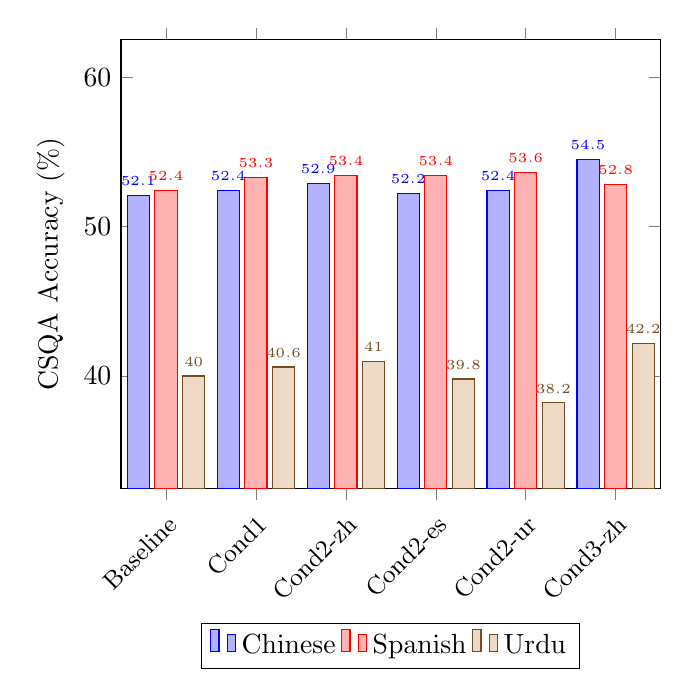
\begin{tikzpicture}
\begin{axis}[
    ybar,
    enlargelimits=0.1,
    legend style={at={(0.5,-0.3)}, anchor=north,legend columns=-1},
    ylabel={CSQA Accuracy (\%)},
    symbolic x coords={Baseline,Cond1,Cond2-zh,Cond2-es,Cond2-ur,Cond3-zh},
    xtick=data,
    xticklabel style={rotate=45, anchor=north east, font=\small},
    nodes near coords,
    nodes near coords align={vertical},
    nodes near coords style={font=\tiny},
    ymin=35,
    ymax=60,
    bar width=8pt,
]
\addplot coordinates {(Baseline,52.1) (Cond1,52.4) (Cond2-zh,52.9) (Cond2-es,52.2) (Cond2-ur,52.4) (Cond3-zh,54.5)};
\addplot coordinates {(Baseline,52.4) (Cond1,53.3) (Cond2-zh,53.4) (Cond2-es,53.4) (Cond2-ur,53.6) (Cond3-zh,52.8)};
\addplot coordinates {(Baseline,40.0) (Cond1,40.6) (Cond2-zh,41.0) (Cond2-es,39.8) (Cond2-ur,38.2) (Cond3-zh,42.2)};
\legend{Chinese,Spanish,Urdu}
\end{axis}
\end{tikzpicture}
\caption{CSQA Native Prompt Accuracy by Condition}
\label{fig:csqa_results}
\end{figure}

\subsection{Label Extraction Methodology}
Initial XNLI scores were significantly affected by label extraction issues that required correction:

\begin{itemize}
\item \textbf{Missing Chinese native labels}: Baseline Chinese XNLI improved from 2.0\% to 35.8\% after adding Chinese label mappings (\texttt{蕴含}/\texttt{蕴涵} for entailment, \texttt{矛盾} for contradiction, \texttt{中立} for neutral).
\item \textbf{Case-sensitive Spanish matching}: Adding case-insensitive matching improved Spanish baseline from 23.8\% to 49.1\%.
\item \textbf{Code leakage extraction}: Urdu outputs containing Legesher code on subsequent lines (e.g., \texttt{contradiction\textbackslash nتعریف main():}) required first-line-only extraction to avoid misclassification.
\end{itemize}

All scores reported in this paper reflect corrected extraction methodology.

\section{Discussion}

\subsection{The Label Bias Problem in XNLI}
The most significant finding is that XNLI at 3.35B parameter scale measures label bias, not natural language inference capability. The model never predicts ``neutral'' across any condition, reducing the task to binary classification. Consequently, accuracy is determined by how well the model's binary bias aligns with the test set's balanced distribution.

This explains several patterns:
\begin{itemize}
\item Chinese baseline (92\% contradiction) scores 35.8\%; Cond 2-zh (65\% entailment) scores 42.3\% — the gain reflects rebalancing, not improved comprehension.
\item Spanish baseline (50\% entailment/50\% contradiction) scores highest (49.1\%) because its balanced bias naturally aligns with the test set.
\item Fine-tuning consistently hurts Spanish because it disrupts this naturally balanced bias.
\end{itemize}

\subsection{Language-Specific Effects}
The keyword-swap comparison (same 5K files, only keywords differ) reveals language-specific effects:
\begin{itemize}
\item Chinese keywords: +6.2pp on XNLI (statistically significant)
\item Spanish keywords: -2.8pp on XNLI (regression)
\item Urdu keywords: +0.9pp on XNLI (no effect)
\end{itemize}

This variation likely reflects differences in tokenizer overlap between code keywords and NLI labels, and differences in the model's pre-existing representation quality for each language.

\subsection{Code Leakage Implications}
Urdu keyword training causes the model to generate Legesher code in response to Urdu prompts — even for non-coding tasks. This indicates that code fine-tuning can contaminate general language generation when the target language lacks established programming language conventions. Urdu has no native programming language; Legesher's keyword translations represent one of the first attempts to create one. The model's conflation suggests caution when fine-tuning on artificially constructed code for languages without native programming traditions.

\subsection{Limitations}
Several limitations constrain this study:
\begin{enumerate}
\item \textbf{Model scale}: Tiny Aya at 3.35B parameters may be too small to benefit from code training in the ways larger models do. Findings may not generalize to larger architectures.
\item \textbf{Incomplete condition coverage}: Only Chinese has Condition 3 (mixed native sources) completed; Spanish and Urdu Condition 3 are not yet evaluated.
\item \textbf{No English benchmark evaluation}: Catastrophic forgetting has not been assessed — the models may have degraded English performance.
\item \textbf{Benchmark limitations}: XNLI proved unsuitable for measuring NLI at this scale; future work should use benchmarks with per-question answer options.
\end{enumerate}

\section{Conclusion} 
\label{sec:conclusion}
Our experimental ladder demonstrates that native-language code provides language-specific benefits, with Chinese keyword-swapped code yielding a +6.2 percentage point improvement on Chinese XNLI. However, deeper analysis reveals that XNLI accuracy at this scale primarily reflects label bias shifts rather than improved natural language inference capability. The model collapses to binary classification, never predicting the ``neutral'' category.

Mathematical reasoning shows no improvement across any condition, confirming that code fine-tuning does not enhance arithmetic capabilities at 3.35B parameter scale. Urdu keyword training causes code leakage into evaluation outputs, highlighting potential risks when fine-tuning on artificially constructed code for languages without native programming traditions.

These findings suggest that while native-language code can influence model behavior, the effects are language-specific and should be interpreted with careful attention to benchmark limitations. Future work should evaluate catastrophic forgetting on English benchmarks, explore larger model scales, and select benchmarks with per-question answer options that resist label bias collapse.

\section{Future Work}
\label{sec:future}

Several directions emerge from this study for subsequent phases of the experiment.

\subsection{English Benchmark Evaluation — Catastrophic Forgetting Check}
A critical next step is evaluating all fine-tuned models on English benchmark data. Currently, every condition has been evaluated on Chinese, Spanish, and Urdu benchmarks, but English benchmarks (MGSM-en, XNLI-en, CSQA-en) remain untested. This evaluation is essential to determine whether multilingual code fine-tuning causes catastrophic forgetting — degradation in English language performance. Several of the strongest results (such as Chinese XNLI improvements) could be undermined if the models simultaneously lose English capability. This check will inform whether the observed gains represent genuine enhancement or merely cross-lingual trade-offs.

\subsection{Extended Condition Evaluation}
Several planned conditions remain incomplete and warrant further investigation:
\begin{itemize}
\item \textbf{Condition 3 for Spanish and Urdu}: Only Chinese Condition 3 (mixed native sources with Wenyan) was completed in this cycle. Spanish and Urdu variants require additional native-language code collection to enable equivalent evaluation.
\item \textbf{Condition 4 — Strictly Native Code}: Evaluating models trained exclusively on code written entirely in native languages (without English-derived content) would reveal whether purely native sources carry unique signal beyond keyword-swapped approaches.
\item \textbf{Condition 5 — Cross-Lingual Transfer}: Experiments training on one language and evaluating on related languages would determine whether shared script or language family creates transfer effects, particularly relevant for Urdu with its Arabic script.
\end{itemize}

\subsection{Benchmark Selection for Future Cycles}
The limitations of XNLI at this model scale suggest that future evaluation cycles should incorporate benchmarks more robust to label bias:
\begin{itemize}
\item \textbf{Belebele}: A 4-way reading comprehension benchmark where each question has unique answer options, making fixed label bias impossible.
\item \textbf{SIB-200}: Topic classification with 7 concrete categories (science, sports, politics, etc.) across 200+ languages, providing concrete labels more learnable than abstract entailment distinctions.
\item \textbf{XStoryCloze}: Already in the evaluation pipeline, this 2-way story completion benchmark with unique endings per question avoids the label collapse seen in XNLI.
\end{itemize}

\subsection{Neutral Label Investigation}
A persistent finding is that the model never predicts ``neutral'' in XNLI across any condition. Future work should investigate whether this represents:
\begin{itemize}
\item A fundamental limitation of 3.35B parameter models for 3-way classification tasks
\item A prompt engineering issue resolvable by explicitly including ``neutral'' as an option in the prompt template
\item A pre-training bias that could be addressed through targeted fine-tuning on balanced NLI data
\end{itemize}

\subsection{Alternative Evaluation Methodologies}
Current evaluation uses open-ended generation with extraction, which revealed complications including code leakage and multi-line outputs. Future evaluations should compare this against log-probability scoring (implemented in \texttt{eval\_pipeline.py}) to determine which method provides more reliable signal for small-scale multilingual models. This is particularly relevant for Urdu, where code contamination significantly affected extraction quality.

\subsection{Larger Model Scale Validation}
The null results for MGSM and the label bias collapse in XNLI may reflect model scale limitations rather than inherent properties of multilingual code fine-tuning. Replicating key conditions with larger models (e.g., 7B or 13B parameters) would determine whether the observed effects scale with model size.

\section{Acknowledgments}
We would like to thank Cohere for providing the opportunity to explore this project through the Expedition Tiny Aya program. Their support and infrastructure were instrumental in enabling this research.

We would also like to acknowledge the open-source community for their contributions to multilingual programming languages and code datasets, especially the Language Decoded Community Dataset \cite{legesher_language_decoded_community}, which was essential for our data curation process.

Finally, we thank our colleagues and peers for their valuable feedback and insights during the development of this paper.

%% Use plainnat to work nicely with natbib. 

\bibliographystyle{plainnat}
\bibliography{references}

\end{document}
